%% LaTeX Paper Template, Flip Tanedo (flip.tanedo@ucr.edu)
%% GitHub: https://github.com/fliptanedo/paper-template-2022

\documentclass[12pt]{article}

%!TEX root = paper.tex
%% FLIP’S PREAMBLE; 
%% Use FlipAdditionalHeader for project-specific packages & macros

% \pdfoutput=1 % for JHEP

%%%%%%%%%%%%%%%%%%%%%%%%%%
%%%  COMMON PACKAGES  %%%%
%%%%%%%%%%%%%%%%%%%%%%%%%%

\usepackage{amsmath}
\usepackage{amssymb}
\usepackage{amsfonts}
\usepackage{graphicx}
\usepackage[utf8]{inputenc}     % inspire bibs
\usepackage{aas_macros}				  % ads bibs
\usepackage{bm}                 % \boldsymbol
\usepackage{amsthm}
\usepackage{microtype}

%%%%%%%%%%%%%%%%%%%%%%%%%%%
%%%  UNUSUAL PACKAGES  %%%%
%%%%%%%%%%%%%%%%%%%%%%%%%%%

%% MATH AND PHYSICS SYMBOLS
%% ------------------------
\usepackage{slashed}				% \slashed{k}
\usepackage{mathrsfs}				% Weinberg-esque letters
\usepackage{bbm}					  % \mathbbm{1} conflict: XeLaTeX 
\usepackage{cancel}					
\usepackage[normalem]{ulem} % for \sout
\usepackage{youngtab}	    	% Young Tableaux

%% CONTENT FORMAT AND DESIGN
%% -------------------------
\usepackage[dvipsnames]{xcolor}
\usepackage[hang,flushmargin]{footmisc} % no footnote indent

\usepackage{fancyhdr}		% preprint number
\usepackage{lipsum}			% block of text 
\usepackage{framed}			% boxed remarks / Next time: use mdframed
                        % https://github.com/marcodaniel/mdframed/blob/master/mdframed.pdf
\usepackage{subcaption}	% subfigures
\usepackage{cite}			  % group cites
\usepackage{xspace}			% macro spacing


%% TABLES IN LaTeX
%% ---------------
\usepackage{booktabs}		% professional tables
\usepackage{nicefrac}		% fractions in tables,
\usepackage{multirow}		% multirow elements in a table
\usepackage{arydshln}		% dashed lines in arrays

%% ARRAY STRETCH: vertical spacing between rows
% \renewcommand{\arraystretch}{1.5} %% put this in main text

%% Other Packages and Notes
%% ------------------------
\usepackage[font=small]{caption} 	% caption font is small
\usepackage{float}         			  % for strict placement e.g. [H]


%%%%%%%%%%%%%%%%%%%%%%%%%%%%%%
%%%  DOCUMENT PROPERTIES  %%%%
%%%%%%%%%%%%%%%%%%%%%%%%%%%%%%

\usepackage[margin=2.5cm]{geometry} % margins
\graphicspath{{figures/}}			      % figure folder
\numberwithin{equation}{section}    % set equation numbering
% \usepackage{marginnote}             % for \marginnote{comment}
% \usepackage{mparhack}               % fix for \marginnote
% \usepackage{marginfix}              % fix for \marginnote
% \usepackage{adjustbox}              % to rescale elements



%% References in two columns, smaller
%% http://tex.stackexchange.com/questions/20758/
\usepackage{multicol}
\usepackage{etoolbox}
\usepackage{relsize}
\patchcmd{\thebibliography}
  {\list}
  {\begin{multicols}{2}\smaller\list}
  {}
  {}
\appto{\endthebibliography}{\end{multicols}}


% Change list spacing (instead of package paralist)
% from: http://en.wikibooks.org/wiki/LaTeX/List_Structures#Line_spacing
% alternative: enumitem package
\let\oldenumerate\enumerate
\renewcommand{\enumerate}{
  \oldenumerate
  \setlength{\itemsep}{4pt}
  \setlength{\parskip}{0pt}
  \setlength{\parsep}{0pt}
}

\let\olditemize\itemize
\renewcommand{\itemize}{
  \olditemize
  \setlength{\itemsep}{4pt}
  \setlength{\parskip}{0pt}
  \setlength{\parsep}{0pt}
}

%% FOR DRAFT EDITING AND DISCUSSION
\usepackage{lineno}
% \linenumbers          %% put this in main text


%%%%%%%%%%%%%%%%%%%%%%%%%%%
%%%  (RE)NEW COMMANDS  %%%%
%%%%%%%%%%%%%%%%%%%%%%%%%%%

%% FOR `NOT SHOUTING' CAPS (e.g. acronyms)
%% ---------------------------------------
\usepackage{scalefnt} 
\newcommand\acro[1]{{\footnotesize #1}}           % acronyms in footnote size


%% COMMON PHYSICS MACROS
%% ---------------------
\renewcommand{\tilde}{\widetilde}                 % tilde over characters
\renewcommand{\text}{\textnormal}	                % text in equations 
\renewcommand{\vec}[1]{\mathbf{#1}}               % vectors are boldface

%% Differential and differential/2pi
% \newcommand{\dbar}{d\mkern-6mu\mathchar'26}     % for d/2pi
\newcommand{\dbar}{d\mkern-6mu\mathchar'26\hspace{-.1em}}    
%% Best practice: Roman differential
\newcommand{\D}[1]{\ensuremath{\operatorname{d}\!{#1}}}
\newcommand{\Dbar}[1]{\operatorname{d}\mkern-10mu\mathchar'26\mkern-2mu{#1}}    % fixed spacing
\newcommand{\ket}[1]{\left|#1\right\rangle}       % <#1|
\newcommand{\bra}[1]{\left\langle#1\right|}       % |#1>
\newcommand*{\trans}{\mkern-1.5mu\mathsf{T}}      % transpose

%% COMMANDS FOR TEMPORARY COMMENTS
%% -------------------------------
\newcommand{\comment}[2]{\textcolor{red}{[\textbf{#1} #2]}}
\newcommand{\flip}[1]{{
	\color{green!50!black}
  \footnotesize
  [\textbf{\textsf{Flip}}: \textsf{#1}]
	}}


%% COMMANDS FOR TOP-MATTER
%% -----------------------
\newcommand{\email}[1]{\href{mailto:#1}{#1}}
\newenvironment{institutions}[1][2em]{\begin{list}{}{\setlength\leftmargin{#1}\setlength\rightmargin{#1}}\item[]}{\end{list}}


%% COMMANDS FOR LATEXDIFF
%% ----------------------
%% see http://bit.ly/1M74uwc
\providecommand{\DIFadd}[1]{{\protect\color{blue}#1}} %DIF PREAMBLE
\providecommand{\DIFdel}[1]{{\protect\color{red}\protect\scriptsize{#1}}}

%% REMARK: use latexdiff option --allow-spaces
%% for \frac, ref: http://bit.ly/1iFlujR
%% Errors with environments? https://tex.stackexchange.com/q/73224

%% USAGE: latexdiff draft.tex revision.tex > diff.tex

%%%%%%%%%%%%%%%%%%%%%
%%%  TITLE DATA  %%%%
%%%%%%%%%%%%%%%%%%%%%

%% PREPRINT NUMBER USING fancyhdr
%% Don't forget to set \thispagestyle{firststyle}
%% ----------------------------------------------
\renewcommand{\headrulewidth}{0pt} 	% no separator
\setlength{\headheight}{15pt} 		% min to avoid fancyhdr warning
\fancypagestyle{firststyle}{
	\rhead{\footnotesize%
	\texttt{\FlipTR}%
	}}

%% TOC overwrites fancyhdr, here's a fix
%% http://tex.stackexchange.com/questions/167828/
\usepackage{etoc}
\renewcommand{\etocaftertitlehook}{\pagestyle{plain}}
\renewcommand{\etocaftertochook}{\thispagestyle{firststyle}}			%% \usepackages
% %!TEX root = paper.tex
%% Update the above with the appropriate root

%% Place additional project-specific macros, package calls here
%% These are called before FlipPreambleEnd.tex so that,
%% for example, they are called before hyperref


%% FIGURE SNIPPIT
% \begin{figure}[tb]
%     \centering
%     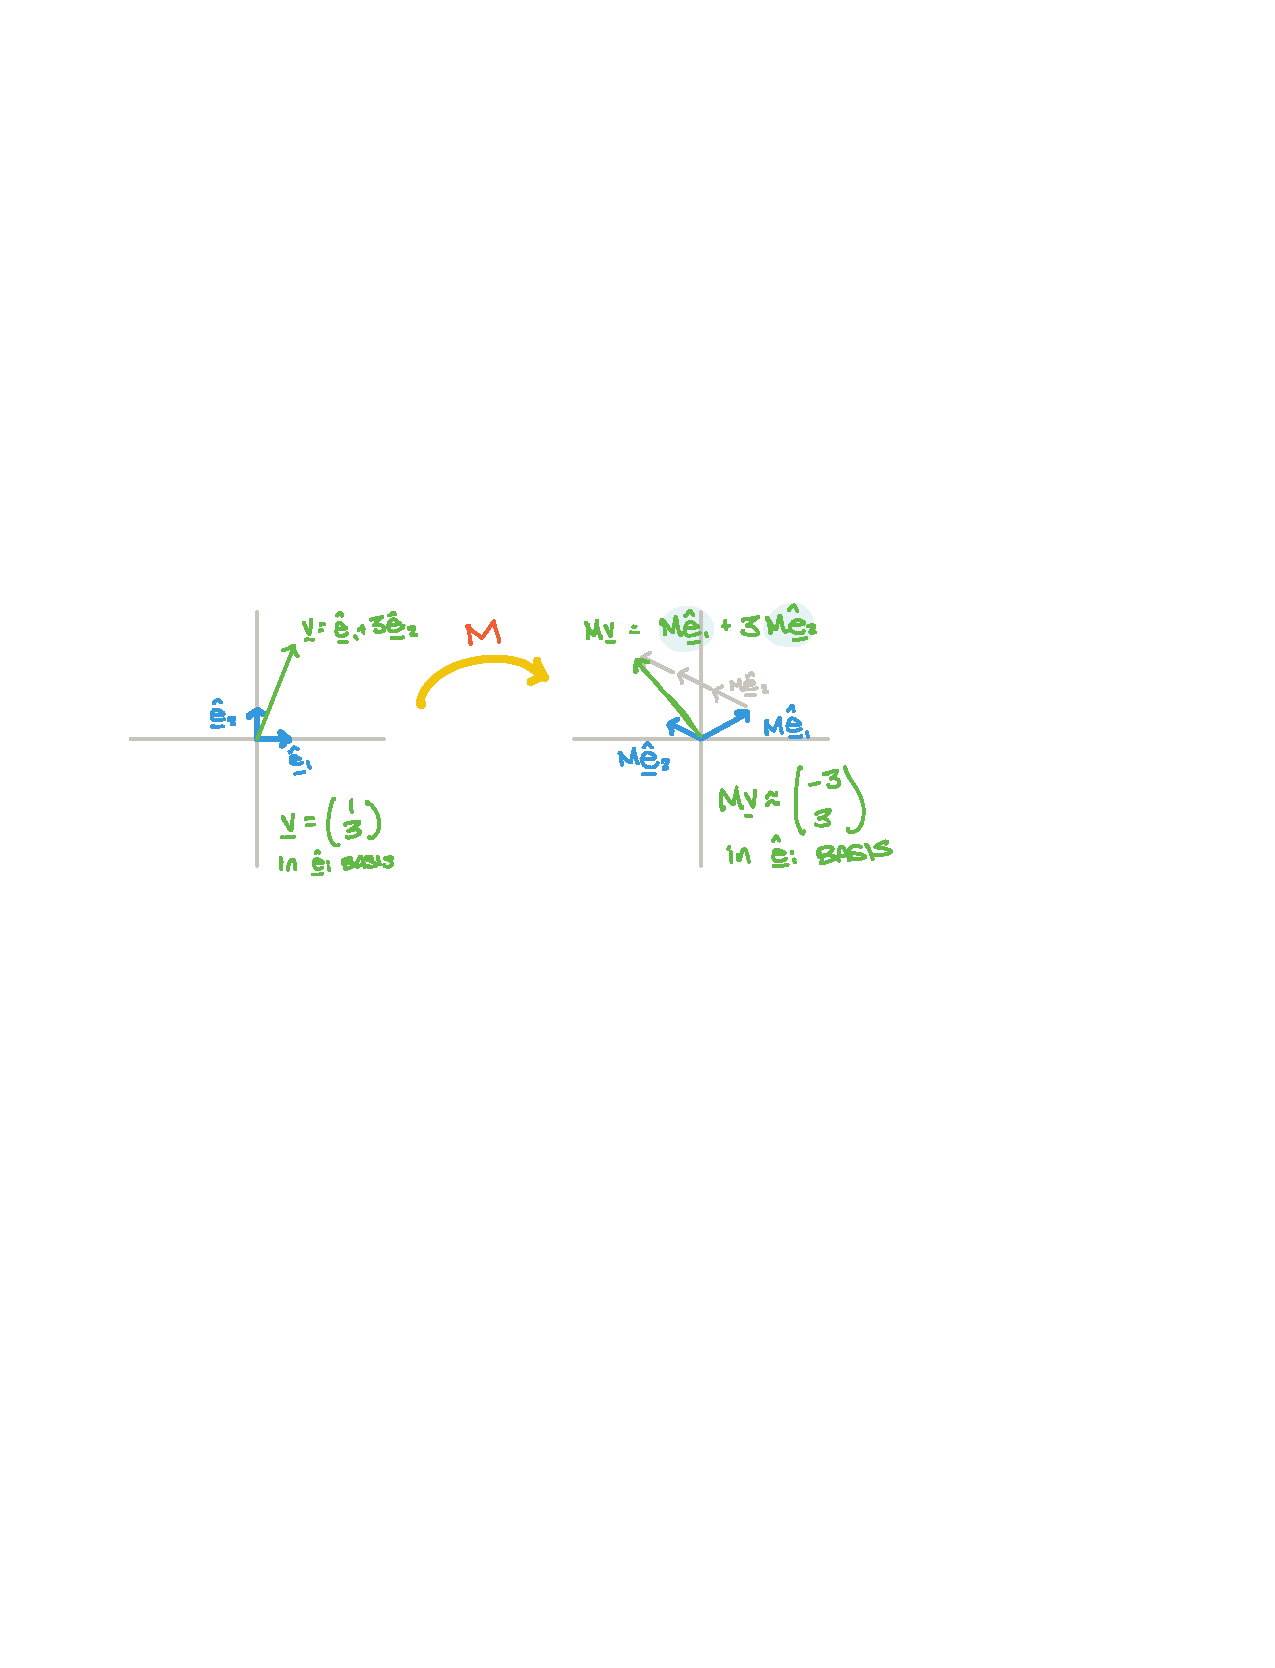
\includegraphics[width=.8\textwidth]{figures/maps_M.pdf}
%     \caption{.}
%     \label{fig:}
% \end{figure}

%% THEOREM ENVIRONMENTS


%% Because mdframed causes a bunch of warnings
%% https://tex.stackexchange.com/questions/64331/disable-warning-from-mdframed 
\usepackage{silence}
\WarningFilter{mdframed}{You got a bad break}
\WarningFilter{mdframed}{correct box splittet fails}



\newmdtheoremenv[
    skipabove=2em,
    skipbelow=2em,
    linewidth=5pt,
    linecolor=red!50!black,
    topline=false,
    rightline=false,
    bottomline=false
    ]{exercise}{Exercise}[section]


\newmdtheoremenv[
    skipabove=2em,
    skipbelow=2em,
    linewidth=5pt,
    linecolor=gray,
    topline=false,
    rightline=false,
    bottomline=false
    ]{example}{Example}[section]

\newmdtheoremenv[
    skipabove=2em,
    skipbelow=2em,
    linewidth=5pt,
    linecolor=blue,
    topline=false,
    rightline=false,
    bottomline=false
    ]{bigidea}{Key Idea}[section]
\newcommand{\bigidearef}{Key~Idea\xspace}
\newcommand{\bigidearefs}{Key~Ideas\xspace}

%% AMS Theorem version
% \newtheorem{exercise}{Exercise}[section]
% \newtheorem{example}{Example}[section]

%% Example: replace YourName with your name
\newcommand{\YourName}[1]{{	
	\color{blue!50!black}\footnotesize
	[\textbf{\textsf{YourName}}: \textsf{#1}]}}


\renewcommand{\tilde}{\widetilde}   % tilde over characters
\renewcommand{\vec}[1]{\mathbf{#1}} % vectors are boldface
\newcommand{\bas}[1]{\hat{\mathbf{#1}}} 	% basis vectors have hat
\newcommand{\row}[1]{\tilde{\mathbf{#1}}} 	% row vectors have tilde

% For matrices
\newcommand{\aij}[2]{^{#1}_{\phantom{#1}#2}}
\newcommand{\mat}[3]{#1\aij{#2}{#3}}
\newcommand{\pp}{\phantom{+}}
\newcommand{\inv}{^{-1}}


\usepackage{pifont}
	\newcommand{\cmark}{\ding{51}}%
	\newcommand{\xmark}{\ding{55}}%


%% COMMANDS FOR TEMPORARY COMMENTS
%% -------------------------------
\newcommand{\comment}[2]{\textcolor{red}{[\textbf{#1} #2]}}
\newcommand{\flip}[1]{{
	\color{green!50!black}
  \footnotesize
  [\textbf{\textsf{Flip}}: \textsf{#1}]
	}}

\newcommand{\correction}[2]{{
	\color{green!50!black}
  \footnotesize
  [\textbf{\textsf{Correction,~#1}}: \textsf{#2}]
	}}
 	%% Use this define additional macros
% %!TEX root = paper.tex
%% Update the above with the appropriate root


%% LISTINGS PACKAGE
%% https://www.overleaf.com/learn/latex/Code_listing
%% https://tex.stackexchange.com/a/350242
\usepackage{xcolor}
\usepackage[most]{tcolorbox}
\usepackage{listings}

\definecolor{white}{rgb}{1,1,1}
\definecolor{mygreen}{rgb}{0,0.4,0}
\definecolor{light_gray}{rgb}{0.97,0.97,0.97}
\definecolor{mykey}{rgb}{0.117,0.403,0.713}

\tcbuselibrary{listings}
\newlength\inwd
\setlength\inwd{1.3cm}

\newcounter{ipythcntr}
\renewcommand{\theipythcntr}{\texttt{[\arabic{ipythcntr}]}}

\newtcblisting{pyin}[1][]{%
  sharp corners,
  enlarge left by=\inwd,
  width=\linewidth-\inwd,
  enhanced,
  boxrule=0pt,
  colback=light_gray,
  listing only,
  top=0pt,
  bottom=0pt,
  overlay={
    \node[
      anchor=north east,
      text width=\inwd,
      font=\footnotesize\ttfamily\color{mykey},
      inner ysep=2mm,
      inner xsep=0pt,
      outer sep=0pt
      ] 
      at (frame.north west)
      {\refstepcounter{ipythcntr}\label{#1}In \theipythcntr:};
  }
  listing engine=listing,
  listing options={
    aboveskip=1pt,
    belowskip=1pt,
    basicstyle=\footnotesize\ttfamily,
    language=Python,
    keywordstyle=\color{mykey},
    showstringspaces=false,
    stringstyle=\color{mygreen}
  },
}
\newtcblisting{pyprint}{
  sharp corners,
  enlarge left by=\inwd,
  width=\linewidth-\inwd,
  enhanced,
  boxrule=0pt,
  colback=white,
  listing only,
  top=0pt,
  bottom=0pt,
  overlay={
    \node[
      anchor=north east,
      text width=\inwd,
      font=\footnotesize\ttfamily\color{mykey},
      inner ysep=2mm,
      inner xsep=0pt,
      outer sep=0pt
      ] 
      at (frame.north west)
      {};
  }
  listing engine=listing,
  listing options={
      aboveskip=1pt,
      belowskip=1pt,
      basicstyle=\footnotesize\ttfamily,
      language=Python,
      keywordstyle=\color{mykey},
      showstringspaces=false,
      stringstyle=\color{mygreen}
    },
}
\newtcblisting{pyout}[1][\theipythcntr]{
  sharp corners,
  enlarge left by=\inwd,
  width=\linewidth-\inwd,
  enhanced,
  boxrule=0pt,
  colback=white,
  listing only,
  top=0pt,
  bottom=0pt,
  overlay={
    \node[
      anchor=north east,
      text width=\inwd,
      font=\footnotesize\ttfamily\color{mykey},
      inner ysep=2mm,
      inner xsep=0pt,
      outer sep=0pt
      ] 
      at (frame.north west)
      {\setcounter{ipythcntr}{\value{ipythcntr}}Out#1:};
  }
  listing engine=listing,
  listing options={
      aboveskip=1pt,
      belowskip=1pt,
      basicstyle=\footnotesize\ttfamily,
      language=Python,
      keywordstyle=\color{mykey},
      showstringspaces=false,
      stringstyle=\color{mygreen}
    },
}


\newtheorem{exercise}{Exercise}[section]
\newtheorem{example}{Example}[section]
%!TEX root = paper.tex
%% These are packages that need to be called at the end of the preamble 
%% or else they may lead to potential package conflicts.

%%%%%%%%%%%%%%%%%%%
%%%  HYPERREF  %%%%
%%%%%%%%%%%%%%%%%%%

%% This package has to be at the end; can lead to conflicts
\usepackage[
	colorlinks=true,
	citecolor=green!50!black,
	linkcolor=NavyBlue!75!black,
	urlcolor=green!50!black,
	hypertexnames=false]{hyperref}

%%%%%%%%%%%%%%%%%%%%%%%%%%%%%%%%%%%%%%%%
%%%  Must be called after HYPERREF  %%%%
%%%%%%%%%%%%%%%%%%%%%%%%%%%%%%%%%%%%%%%%


\usepackage{orcidlink}			% orcid ID icon; after hyperref
\usepackage{cleveref}
\crefformat{equation}{(#2#1#3)}	% strip eq.~ 
\crefrangeformat{equation}{(#3#1#4\,--\,#5#2#6)} % strip eqs.~			%% packages that have to be at the end
\begin{document}

\newcommand{\FlipTR}{UCR-TR-2023-FLIP-00X} % (pdfsync may fail on 1st page)
	\thispagestyle{firststyle} 	% TR#; otherwise use \thispagestyle{empty}


%%%%%%%%%%%%%%%%%%%%%%%%
%%%  FRONTMATTER    %%%%
%%%%%%%%%%%%%%%%%%%%%%%%

\begin{center}
    {\huge \textbf{Machine Learning for Physics Students} \par}
    \vskip .5cm
    %!TEX root = paper.tex
%% Update the above with the appropriate root

%% This is the author list
%% We separate it to keep the main file clean; this is
%% not the part of the document that gets updated often.

\newcommand{\authorA}{Flip Tanedo}
\newcommand{\emailA}{flip.tanedo@ucr.edu}
\newcommand{\orcidA}{0000-0003-4642-2199}
\newcommand{\institutionA}{
		Department of Physics \& Astronomy, 
	    University of  California, Riverside, 
	    \acro{CA} 92521}

\newcommand{\authorB}{Your Name}
\newcommand{\emailB}{your.name@ucr.edu}
\newcommand{\orcidB}{0000-0003-4642-2200}
\newcommand{\institutionB}{
		Department of Physics \& Astronomy, 
	    University of  California, Elsewhere, 
	    \acro{CA} 99999}

\newcommand{\authorC}{Tu Nombre}
\newcommand{\emailC}{tu.nombre@ucr.edu}
\newcommand{\orcidC}{0000-0003-4642-2201}
\newcommand{\institutionC}{
		Department of Physics \& Astronomy, 
	    University of  California, Elsewhere, 
	    \acro{CA} 99999}

	\textbf{\authorA}%$^{a}$,
	% \textbf{\authorB}$^{b}$,
	% and
	% \textbf{\authorC}$^{c}$, 
	\\ 
	\texttt{\footnotesize \email{\emailA}}~\orcidlink{\orcidA}%,
	% \texttt{\footnotesize \email{\emailB}}~\orcidlink{\orcidB},
	% \texttt{\footnotesize \email{\emailC}}~\orcidlink{\orcidC}

	\vspace{-.8em}
    \begin{institutions}[1.7cm]
    \footnotesize
    { 
    	% $^{a}$
    	\textit{\institutionA} 
    	% \\ $^{b}$ \textit{\institutionB} 
    	% \\ $^{c}$ \textit{\institutionC} 
	}    
    \end{institutions}


\end{center}

\begin{abstract}
\noindent 
Notes on machine learning for physicists who do not know anything.
\end{abstract}

\small
\setcounter{tocdepth}{2}
\tableofcontents
\normalsize
%\clearpage


%%%%%%%%%%%%%%%%%%%%%
%%%  THE CONTENT  %%%
%%%%%%%%%%%%%%%%%%%%%

% Some examples that I'd like to keep handy
% \section{Examples}
% %!TEX root = paper.tex
%% Update the above with the appropriate root

\section{Macros}
\label{sec:macros}

\flip{This is a comment. Let's test out the `not shouting' caps:}
\begin{itemize}
	\item \acro{AdS} in \acro{5D} at the \acro{LHC}.
	\item AdS in 5D at the LHC. 
	\item A third list item to test list spacing.
\end{itemize}


\section{Figures in Equation Environments}
\label{sec:figs}

\begin{align}
	\vcenter{
		\hbox{\includegraphics[width=.1\textwidth]{{example-image-a}}}
		}
	&=
	i g \gamma^\mu \ . 
	\label{eq:vector}
	\\
	\vcenter{
		\hbox{\includegraphics[width=.1\textwidth]{{example-image-a}}}
		}
	&=
	g \gamma^\mu\gamma^5 \ . 
	\label{eq:axial}
	\\
	\vcenter{
		\hbox{\includegraphics[width=.1\textwidth]{{example-image-a}}}
		}
	&=
	ig  \ . 
	\label{eq:scalar}
	\\
	\vcenter{
		\hbox{\includegraphics[width=.1\textwidth]{{example-image-a}}}
		}
	&=
	g \gamma^5 \ . 
	\label{eq:pseudo}
\end{align}

\section{Best practices for tables}
\label{sec:tables}

% \begin{table}
	% \renewcommand{\arraystretch}{1.3} % spacing between rows
	% \centering
	\begin{tabular}{ @{} llll @{} } \toprule % @{} removes space
		Element & Core MF & Mantle MF & $C_\text{cap}^N (\text{s}^{-1})$ 
		\\ \hline
		Iron & 0.855 & 0.0626 & $9.43\times 10^{7}$ 
		\\
		Nickel & 0.052 & 0.00196 & $7.10\times 10^{6}$ 
		\\
		Silicon & 0.06 & 0.210 & $2.24\times 10^{6}$ 
		\\
		Magnesium & 0 & 0.228 & $1.05\times 10^{6}$ 
		\\ \bottomrule
	\end{tabular}
	% \caption{
		% Mass fractions of the Earth's core and mantle.
		% \label{table:elements}
% 	}
% \end{table}

\section{cleveref}
\label{sec:cleveref}

\texttt{cleveref} is a handy package when referring to ranges of equations. 

The pseudoscalar rule is:
\begin{itemize}
	\item Using \texttt{amsmath.sty}'s \texttt{eqref}: \eqref{eq:pseudo}
	\item Using \texttt{cleverefs}'s \texttt{cref}: \cref{eq:pseudo}
\end{itemize}

The equations above are
\begin{itemize}
	\item Using \texttt{amsmath.sty}'s \texttt{eqref}: \eqref{eq:vector} -- \eqref{eq:pseudo}
	\item Using \texttt{cleverefs}'s \texttt{crefrange}: \crefrange{eq:vector}{eq:pseudo}
\end{itemize}

The equations above are (glomped together)
\begin{itemize}
	\item Using \texttt{amsmath.sty}'s \texttt{eqref}: \eqref{eq:vector}, \eqref{eq:axial}, \eqref{eq:scalar}, \eqref{eq:pseudo}
	\item Using \texttt{cleverefs}'s \texttt{cref}: \cref{eq:vector,eq:pseudo,eq:axial,eq:scalar}
\end{itemize}

The sections above are \cref{sec:macros,sec:cleveref,sec:figs,sec:tables}.

\section{Other Best Practices}


\subsection{Kerning: spacing between characters}
Math operators have a natural spacing before and after depending on the context. In the following example, spaces indicate that the coefficient $a$ multiplies the logarithm of $b$:
\begin{align}
	a\log b && a\log(bc)
\end{align}
The space on either side of $\log$ indicate that $\log$ is a mathematical operator. The second example still has the space between $a$ and $\log$, but has no space between $\log$ and $(bc)$ because the parenthesis belongs to the mathematical function.\footnote{Example from \url{https://tex.stackexchange.com/a/140647}}

You can use \textbackslash\texttt{operatorname} and \textbackslash\texttt{DeclareMathOperator} for functions that are not built in.

\subsection{Upright characters}
These come from the \acro{ISO 80000} standards for typesetting mathematics and physics.\footnote{See discussion in \url{https://tex.stackexchange.com/questions/14821/whats-the-proper-way-to-typeset-a-differential-operator}} It is not obvious to me that these are applicable to the typographical culture of physics, but the most important thing is to be consistent.
\begin{itemize}
	\item Units are always upright, \textmu m is a micrometer. You can use various unit packages to do this automatically. 
	\item The base of the natural logarithm is upright $\mathrm{e}^{i\pi}$ versus $e^{i\pi}$.
	\item The differential is an operator so it should be upright. I have macros for this: $dx$ vs.~$\D{x}$ and $\dbar p$ vs.~$\Dbar{p}$. The \texttt{physics} package has macros for this. 
\end{itemize}
There is a historical discussion on hsm.stackexchange\footnote{\url{https://hsm.stackexchange.com/questions/6727/fracdydx-versus-frac-mathrm-dy-mathrm-dx}}.


\subsection{Ranges}

Hyphens, en dashes, em dashes, and minus signs in math mode are all grammatically different.
\begin{itemize}
	\item En dashes replace hyphens in a compound adjective where one of the elements is a two-word compound: `post--Cold War era.'\footnote{From \url{https://www.merriam-webster.com/words-at-play/em-dash-en-dash-how-to-use}}
	\item En dashes are used for combinations of two names in place of the wordd `and'. Randall--Sundrum model.
	\item For compound names of a single person, use a hyphen: Levi-Civita.
\end{itemize}

\subsection{Inserting code}

Uncomment the following as well as the lines in \texttt{paper.tex} that loads the \texttt{listings} package.
% %!TEX root = paper.tex
%% Update the above with the appropriate root

\section{Code example}

These are examples of the \texttt{listings} package for typesetting code. See Overleaf\footnote{\url{https://www.overleaf.com/learn/latex/Code_listing}} and tex.stackexchange\footnote{\url{https://tex.stackexchange.com/a/350242}} for discusisons.

\subsection{Basic Example}
\begin{pyin}
print("Hello world")
\end{pyin}

\begin{pyprint}
Hello world
\end{pyprint}

\subsection{Outputs and returned values}
And here we also have a return value in the last line of the input cell.
\begin{pyin}[labelOfTheSecondInput]
def twicify(arg):
    print("Received:", arg, "- Will double now...")
    return 2 * arg
twicify(1)
\end{pyin}

\begin{pyprint}
Received: 1 - Will double now...
\end{pyprint}

\begin{pyout}
2
\end{pyout}

\subsection{Referencing input}
You can also reference the labeled input \ref{labelOfTheSecondInput}, from above.
\begin{pyin}
"and the counter will automatically do the right thing :)"
\end{pyin}
\begin{pyout}
'and the counter will automatically do the right thing :)'
\end{pyout}




\subsection{Miscellaneous}

\begin{itemize}
	\item \textbf{align environment}: Use the \texttt{align} environment instead of \texttt{eqnarray}. See TeXblog discussion\footnote{\url{https://texblog.net/latex-archive/maths/eqnarray-align-environment/}}
	\item \textbf{centering environment}: Use \textbackslash\texttt{centering} rather than the \texttt{center} environment in figure environments to avoid adding extra vertical space.\footnote{\url{https://tex.stackexchange.com/questions/23650/when-should-we-use-begincenter-instead-of-centering}}
	\item \textbf{Roman Subscripts}: use Roman style (e.g.~\textbackslash \texttt{text}\{$\cdots$\}) when the subscript is not a mathematical character. For example, $x_a$ makes sense for the value of $x$ at point $a$, but $x_\text{b}$ should be used if the `b' is shorthand for boundary. Similarly, $E_\text{max}$ for the maximum energy, rather than $E_{max}$.
	\item Spacing: thin\,space, medium\:space, thick\;space, thin\!negative\!space.
	\item \textbf{Ties} (tildes): \LaTeX interprets periods as full stops (end of a sentence). It places extra space after the full stop. Use a tie when a period is not a full stop: Mr.~Roboto versus Mr. Roboto. 
	\item You can also use ties this whenever you want to prevent a line break between words. \LaTeX interprets the tied words as a single word.
	\item The double dollar sign notation for \texttt{displaymath} is depreciated.\footnote{\url{https://tex.stackexchange.com/questions/503/why-is-preferable-to}}
	\item Use $\mid$ instead of pipe for conditions: $p(x\mid y)$ versus $p(x|y)$.
	\item Transpose: The \acro{ISO}~80000 standard has suggestions. $A^T$ vs $A^\top$ vs $A\trans$
\end{itemize}

More information available here:
\begin{itemize}
	\item Consistent typography on tex.stackexchange\footnote{\url{https://tex.stackexchange.com/questions/29840/consistent-typography}}
	\item List of best practices references on tex.stackexchange\footnote{\url{https://tex.stackexchange.com/questions/577/best-practices-references}}, including the list of obsolete packages and commands in 2e\footnote{\url{https://www.ctan.org/tex-archive/info/l2tabu/english/}}
	\item There is an \acro{ISO} standard for typesetting mathematics and physics. As of 2023 it is \acro{ISO\~80000}.
	\item ``The Art of \LaTeX,'' a list of guidelines from Fan Pu Zeng\footnote{\url{https://fanpu.io/blog/2023/latex-tips/}}
	\item Showcase of beautiful typography in \LaTeX\footnote{\url{https://tex.stackexchange.com/questions/1319/showcase-of-beautiful-typography-done-in-tex-friends}}
\end{itemize}



\section{Introduction}

\subsection{Line fitting}

Suppose you know that some data follows a linear relationship,
\begin{align}
    y = ax \ .
\end{align}
% Perhaps you have a circuit where you can set the voltage difference between two points ($x$) and measure the current between those two points ($y$). By Ohm's law, the constant $a$ is the inverse of the resistance, $a = R^{-1}$. Suppose we want to measure the [inverse] resistance. To do this, all we have to do is set the voltage difference to be some convenient value, $x_1$, and then measure what the current is, $y_1$. To be clear, $x$ and $y$ are variables, while $x_1$ and $y_1$ are measured values of these variables in a specific circuit. We deduce that for this circuit $a = y_1/x_1$. 
Suppose $x$ is something that we can control experimentally, like the voltage between two points on a circuit. Further, suppose that $y$ is something that we can measure experimentally, like the current between those two points.  We could then deduce the value of $a$ (the inverse resistance) by picking some value of $x=x_1$ and measuring the corresponding output $y=y_1$, then taking the ratio $a = y_1/x_1$.

% put units on this

Let us now recall that we do not live in a platonic world of idealized measurements. Our measurements are noisy. This means that the ``true'' values of $\hat y_1$ and $\hat x_1$ are different by the measured values. The difference is \emph{random}. If you want to be fancy, we can say that the difference is \textbf{stochastic}, which means that it is random but drawn from a probability distribution. Physicists are trained to be comfortable with stochasticity since it comes up in at least three ways in our education:
\begin{enumerate}
    \item Experimental measurements have finite resolution and suffer from experimental noise. 
    \item Thermodynamic measurements, even idealized ones, are subject to thermal randomness.
    \item Quantum measurements, even idealized ones, are subject to intrinsic quantum randomness.
\end{enumerate}

In order to determine the value of the parameter $a$, we may thus make several measurements. We can dress this act with some sophisticated words about averaging over the randomness so that for large number of measurements $(x_i, y_i)$ we expect that the average value of $y_i/x_i$ to be the `true' value of $a$. Here $i$ indexes each datum so that it ranges from 1 to $N$, the number of $(x,y)$ pairs that we measure in our lab notebook.

Now let us make the situation a bit more interesting. Suppose we have data $\{(x_i, y_i)\}$. We do not know if this data has a linear relationship of the form $y=ax$, but we would like to figure out the value of $a$ and quantify how well the line fits the data. In a completely unrealistic twist, let us further handicap ourselves by saying that we cannot take the quotient $y_i/x_i$. Instead, we have to determine $a$ by guessing several values $a_\text{guess}$ and checking how good the line $y=a_\text{guess} x$ fits the data. 

Suppose we have a list of guesses, $a_I$ where $I=1, \cdots, N_\text{guess}$. How do we quantify how good $y=a_I x$ fits the data? One way is to take each data point and check how well the following relation holds:
\begin{align}
    y_i \stackrel{?}{=} a_I x_i \ ,
\end{align}
which is what we would expect if (1) the data is fit by a linear relationship and (2) $a_I$ is the linear coefficient. One nice comparison is to take each data point indexed by $i$, square the difference between the observed output $y_i$ and the expected output $a_I x_i$, and then sum these squares:
\begin{align}
    L(a) = \sum_i \left(y_i - a x_i\right)^2 \ .
\end{align}
To be fancy let us call $L(a_I)$ the \textbf{loss function} for the hypothesis $a=a_I$.  We could have used $|y_i - a x_i|$, or $\left(y_i - a x_i\right)^{10}$, or any other function that monotonically increases. We should not use $(y_i-a x_i)$ because the sum can end up being small because of large differences with opposite signs. We want to sum over $i$ because this lets us account for all of the data.\footnote{If we replace the sum by a product, for example, then fitting really well to one data point will make the entire loss function small, even if the rest of the data is a poor fit.}

The best value of $a$ from the set of points $\{a_I\}$ is
\begin{align}
    a_\text{best} = \text{arg}\,\text{min}_{a_I} L(a_I) \ ,
\end{align}
where the right hand side means the value of $a_I$ that minimizes the loss function. An algorithm may look like:
\begin{enumerate}
    \item Start with $I=1$. Calculate $L(a_I)$. Write it down.
    \item Advance $I\to I+1$. Calculate $L(a_{I+1})$. Write it down.
    \item Repeat the previous step until you have all $\{L(a_I)\}$.
    \item Pick the smallest value of $L(a_I)$. Return the value of $a_I$ associated with this value of $I$. 
\end{enumerate}
This is not particularly sophisticated and the task is readily offloaded to a computer.

\begin{exercise}
Argue that this procedure generalizes to higher-dimensional linear relationships of the form $\vec{y} = A \vec{x}$ where $\vec{y}$ and $\vec{x}$ are vectors---not necessarily of the same dimension---and $A$ is a matrix of the appropriate dimension. 
\end{exercise}


Just because we have found the \emph{best} fit for the parameter $a$, that does not mean we have found a \emph{good} fit. The value of $L(a)$ for our best fit quantifies how good the $y=ax$ ansatz represents the data. 


If $L(a)$ is very large, perhaps we have not allowed the algorithm to find a reasonable value of $a$. This may be because we did not consider a large enough set of possible $a$ values, since $a$ is drawn from an infinite continuum of possible values. We can then phrase our problem with respect to the continuum of $a$ values: the best fit value of $a$ is the one that minimizes the loss for \emph{fixed data} and \emph{variable a}: $L(a)$. One necessary condition for this is $L'(a) = 0$. At this point you should be thinking about minima versus maxima and local versus global. Further, you should think that we can still offload this task to a computer through clever discrete approximations of continuous problems. One last observation you should make is that for any value of $a$ with $L'(a)\neq 0$, the sign and magnitude of $L'(a)$ gives you information for what direction you should perturb $a$ to approach a minimum. This is because a Taylor expansion tell sus
\begin{align}
    L(a) = L(a_0) + L'(a_0) \Delta a + \cdots .
\end{align}
So if $L'(a_0)$ is large, that means $\Delta a = (a-a_0) <0$ will make $L(a) < L(a_0)$ to leading order. This is the basis for the standard optimizer in basic machine learning, gradient descent.


\emph{However}, it may be that $L_I$ is large for any value of $a$. This indicates that the data is not described by a linear relationship. 

\subsection{Curve Fitting}

\textbf{Regression} is procedure of finding a functional relationship between a dependent variable ($y$) to an independent variable ($x$) using data (pairs $(x,y)$). For humans, this usually means writing an explicit function whose parameters mean something significant. 

\subsection{Representations of Functions}

Vectors







 \section*{Acknowledgments}

\acro{PT}\ thanks 
\emph{your name here}
for useful comments and discussions. 
%
\acro{PT} thanks 
    the Aspen Center for Physics (\acro{NSF} grant \acro{\#1066293})
    % and the Kavli Institute for Theoretical Physics (\acro{NSF} grant \acro{PHY-1748958})
    for 
    its 
    % their
    hospitality during a period where part of this work was completed. 
%
% \acro{PT} is supported by the \acro{DOE} grant \acro{DE-SC}/0008541.
\acro{PT} is supported by a \acro{NSF CAREER} award (\#2045333).

%% Appendices
% \appendix


%% Bibliography
%\bibliographystyle{utcaps} 	% arXiv hyperlinks, preserves caps in title
%\bibliographystyle{utphys} 	% arXiv hyperlinks
% \bibliography{bib title without .bib}

\end{document}